This chapter outlines the requirement specification of the system. This section describes the requirement analysis process. The process of gathering the requirements was done in collaboration with Tromsø IL.

\section{Overview}

The requirements evolved during the process of developing the system. Initially a requirement specification was designed from our perspective. We looked at the different analyze systems out there and as mentioned in chapter 3 a good system for locating key players in opponent teams was lacking. Rather than going very wide providing all kind of analyses we narrowed it down to a very concrete system. A system that tries to to for many things may fell between two chairs, and at the end of the day not providing anything. You spend less time on each feature as you have more features thus reducing the quality on each feature.

The imagined system shall give you the key players in the offensive play of a given opponent soccer team. You shall be able to search on teams and individual players. Additionally you shall be able to see which areas of the pitch players are creating goal chances from. The system also needs a way of capturing data. This shall be an interface that enables you to store successful attacks for any match.

\begin{figure}[ht!]
\centering
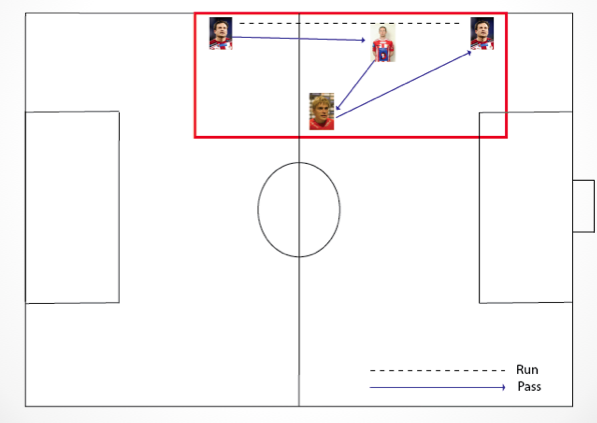
\includegraphics[width=50mm]{images/general/illustration_after_search.png}
\caption{Visioned illustration displaying key players and how they combine given you have queried on a team}
\label{overflow}
\end{figure}

\begin{figure}[ht!]
\centering
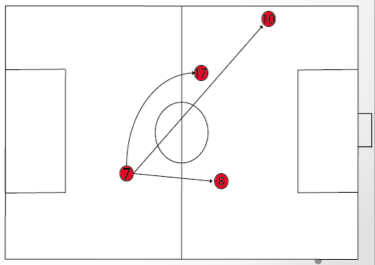
\includegraphics[width=50mm]{images/general/illustration_after_search2.png}
\caption{Visioned illustration of typical passes for a player}
\label{overflow}
\end{figure}

\section{Capture}

A domain model for the captured data is crucial to set early and don't change it radically. Initially we wanted to build a database of all the matches in the Norwegian premier league. From each match every successful attack a team makes should be captured. From the attack started you registrate where the attack started, every pass with from position to the new position, and type of attack. At last if there is a breaking point in the attack this should be captured. The breaking point of the attack is stored with a breakthrough player and what type of breakthrough it was.

Definition of breakthrough player: A player that does something extra that unbalance the other team. This can be a dribble past 1-2 players or a genius pass that opens deference of the opponents team. 

First problem was how to divide the pitch into zones. As we are looking for which zones the breaking point of the attack this is crucial for the searches on the data captured later on. During the development of the system several types of dividing was presented to the coaching staff. 

\begin{figure}[ht!]
\centering
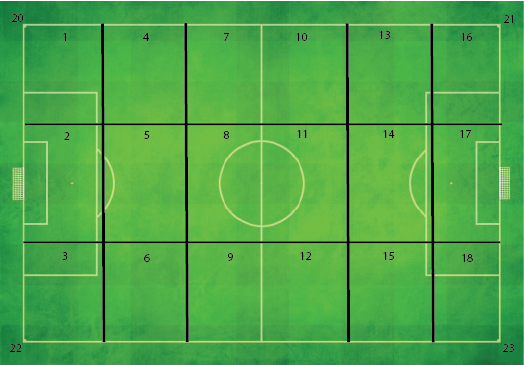
\includegraphics[width=100mm]{images/general/first_zones.png}
\caption{Dividing of pitch - the first suggestion had 18 zones. The team attacking attacks from left to right}
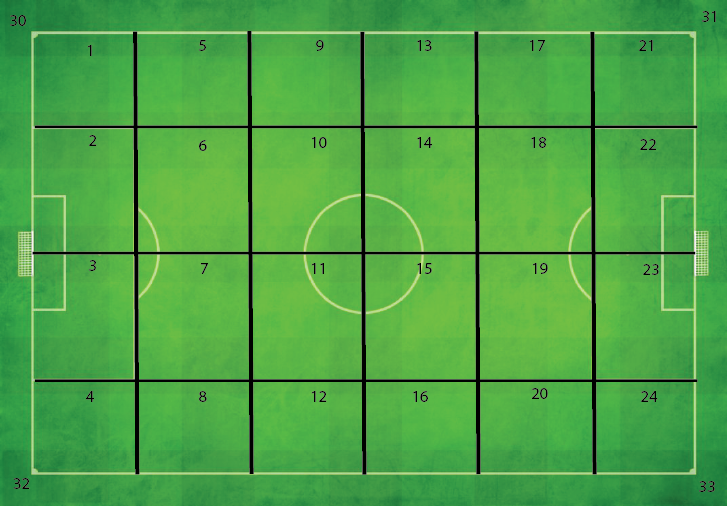
\includegraphics[width=100mm]{images/general/second_zones.png}
\caption{Dividing of pitch - the second suggestion had 18 zones. The team attacking attacks from left to right}
\label{overflow}
\end{figure}

\section{Present}